\documentclass{article}
\usepackage{booktabs}
%\usepackage{ctex}
\usepackage{fancyhdr}
\usepackage{extramarks}
\usepackage{amsmath}
\usepackage{amsthm}
\usepackage{amsfonts}
\usepackage{tikz}
\usepackage[plain]{algorithm}
\usepackage{algpseudocode}
\usepackage{extarrows}
\usepackage{indentfirst}

\usepackage[titletoc]{appendix}
\usepackage{pythonhighlight}
\usepackage{listings}
\usepackage[framed,numbered,autolinebreaks,useliterate]{mcode}

\usetikzlibrary{automata,positioning}

%
% Basic Document Settings
%

\topmargin=-0.45in
\evensidemargin=0in
\oddsidemargin=0in
\textwidth=6.5in
\textheight=9.0in
\headsep=0.25in

\linespread{1.1}

\pagestyle{fancy}
\lhead{\hmwkAuthorName}
\chead{\hmwkClass\ : \hmwkTitle}
\rhead{}
\lfoot{\lastxmark}
\cfoot{\thepage}

\renewcommand\headrulewidth{0.4pt}
\renewcommand\footrulewidth{0.4pt}

\setlength\parindent{2em}

%
% Create Problem Sections
%



\setcounter{secnumdepth}{0}
\newcounter{partCounter}
\newcounter{homeworkProblemCounter}
\setcounter{homeworkProblemCounter}{1}
\nobreak\extramarks{Problem \arabic{homeworkProblemCounter}}{}\nobreak{}

%
% Homework Problem Environment
%
% This environment takes an optional argument. When given, it will adjust the
% problem counter. This is useful for when the problems given for your
% assignment aren't sequential. See the last 3 problems of this template for an
% example.
%


%
% Homework Details
%   - Title
%   - Due date
%   - Class
%   - Section/Time
%   - Instructor
%   - Author
%

\newcommand{\hmwkTitle}{Numerical Differentiation and Integration}
\newcommand{\hmwkDueDate}{May, 2022}
\newcommand{\hmwkClass}{Chap 4}
\newcommand{\hmwkClassTime}{}
\newcommand{\hmwkClassInstructor}{}
\newcommand{\hmwkAuthorName}{\textbf{Yuchen Ge}}

%
% Title Page
%

\title{
    \vspace{2in}
    \textmd{\textbf{\hmwkClass:\ \hmwkTitle}}\\
    \normalsize\vspace{0.1in}\small{Due\ on\ \hmwkDueDate\ }\\
    \vspace{0.1in}\large{\textit{\hmwkClassInstructor\ \hmwkClassTime}}
    \vspace{3in}
}

\author{\hmwkAuthorName}
\date{}

\renewcommand{\part}[1]{\textbf{\large Part \Alph{partCounter}}\stepcounter{partCounter}\\}

%
% Various Helper Commands
%

% Useful for algorithms
\newcommand{\alg}[1]{\textsc{\bfseries \footnotesize #1}}

% For derivatives
\newcommand{\deriv}[1]{\frac{\mathrm{d}}{\mathrm{d}x} (#1)}

% For partial derivatives
\newcommand{\pderiv}[2]{\frac{\partial}{\partial #1} (#2)}

% Integral dx
\newcommand{\dx}{\mathrm{d}x}

% Alias for the Solution section header
\newcommand{\solution}{\textbf{\large Solution}}

% Probability commands: Expectation, Variance, Covariance, Bias
\newcommand{\C}{\mathrm{C}}
\newcommand{\D}{\mathrm{D}}
\newcommand{\E}{\mathrm{E}}
\newcommand{\U}{\mathrm{U}}
\newcommand{\Z}{\mathbb{Z}}
\newcommand{\R}{\mathbb{R}}
\newcommand{\Q}{\mathbb{Q}}
\newcommand{\N}{\mathbb{N}}
\begin{document}
\maketitle

\pagebreak
\section{1. Introduction}

The chapter mianly deals with the problem of numerical differentiation and integration. \textbf{When dealing with numerical differentiation}, we have the three(five)-point midpoint(endpoint) formulas. \textbf{When dealing with numerical integration}, we have closed (open) newton-cotes formulas, composite numerical integration, romberg integration, gaussian quadrature, multiple integration via former techniques.

First we claim that all function and variable names are self-clear. And a/b is interpreted to be section a question b, e.g. 4.4/7.

\section{2. Application of Five-point Formulas (4.1/5a)}

\subsection{2.1 Program Running and Data Analysis}
    
    The question requires the best approximation of the differentiation. Thus we apply five-point midpoint(endpoint) fomulas for the best approximation. Considering the data types we apply the five-point endpoint formulas (4.7) for solving $x=2.1,2.2,2.5,2.6$ and the five-point midpoint formulas (4.6) for solving $x=2.3,2.4$. We run the program as follows. (Meanwhile we display the running time.)
    \begin{figure}[h]
    \centering
    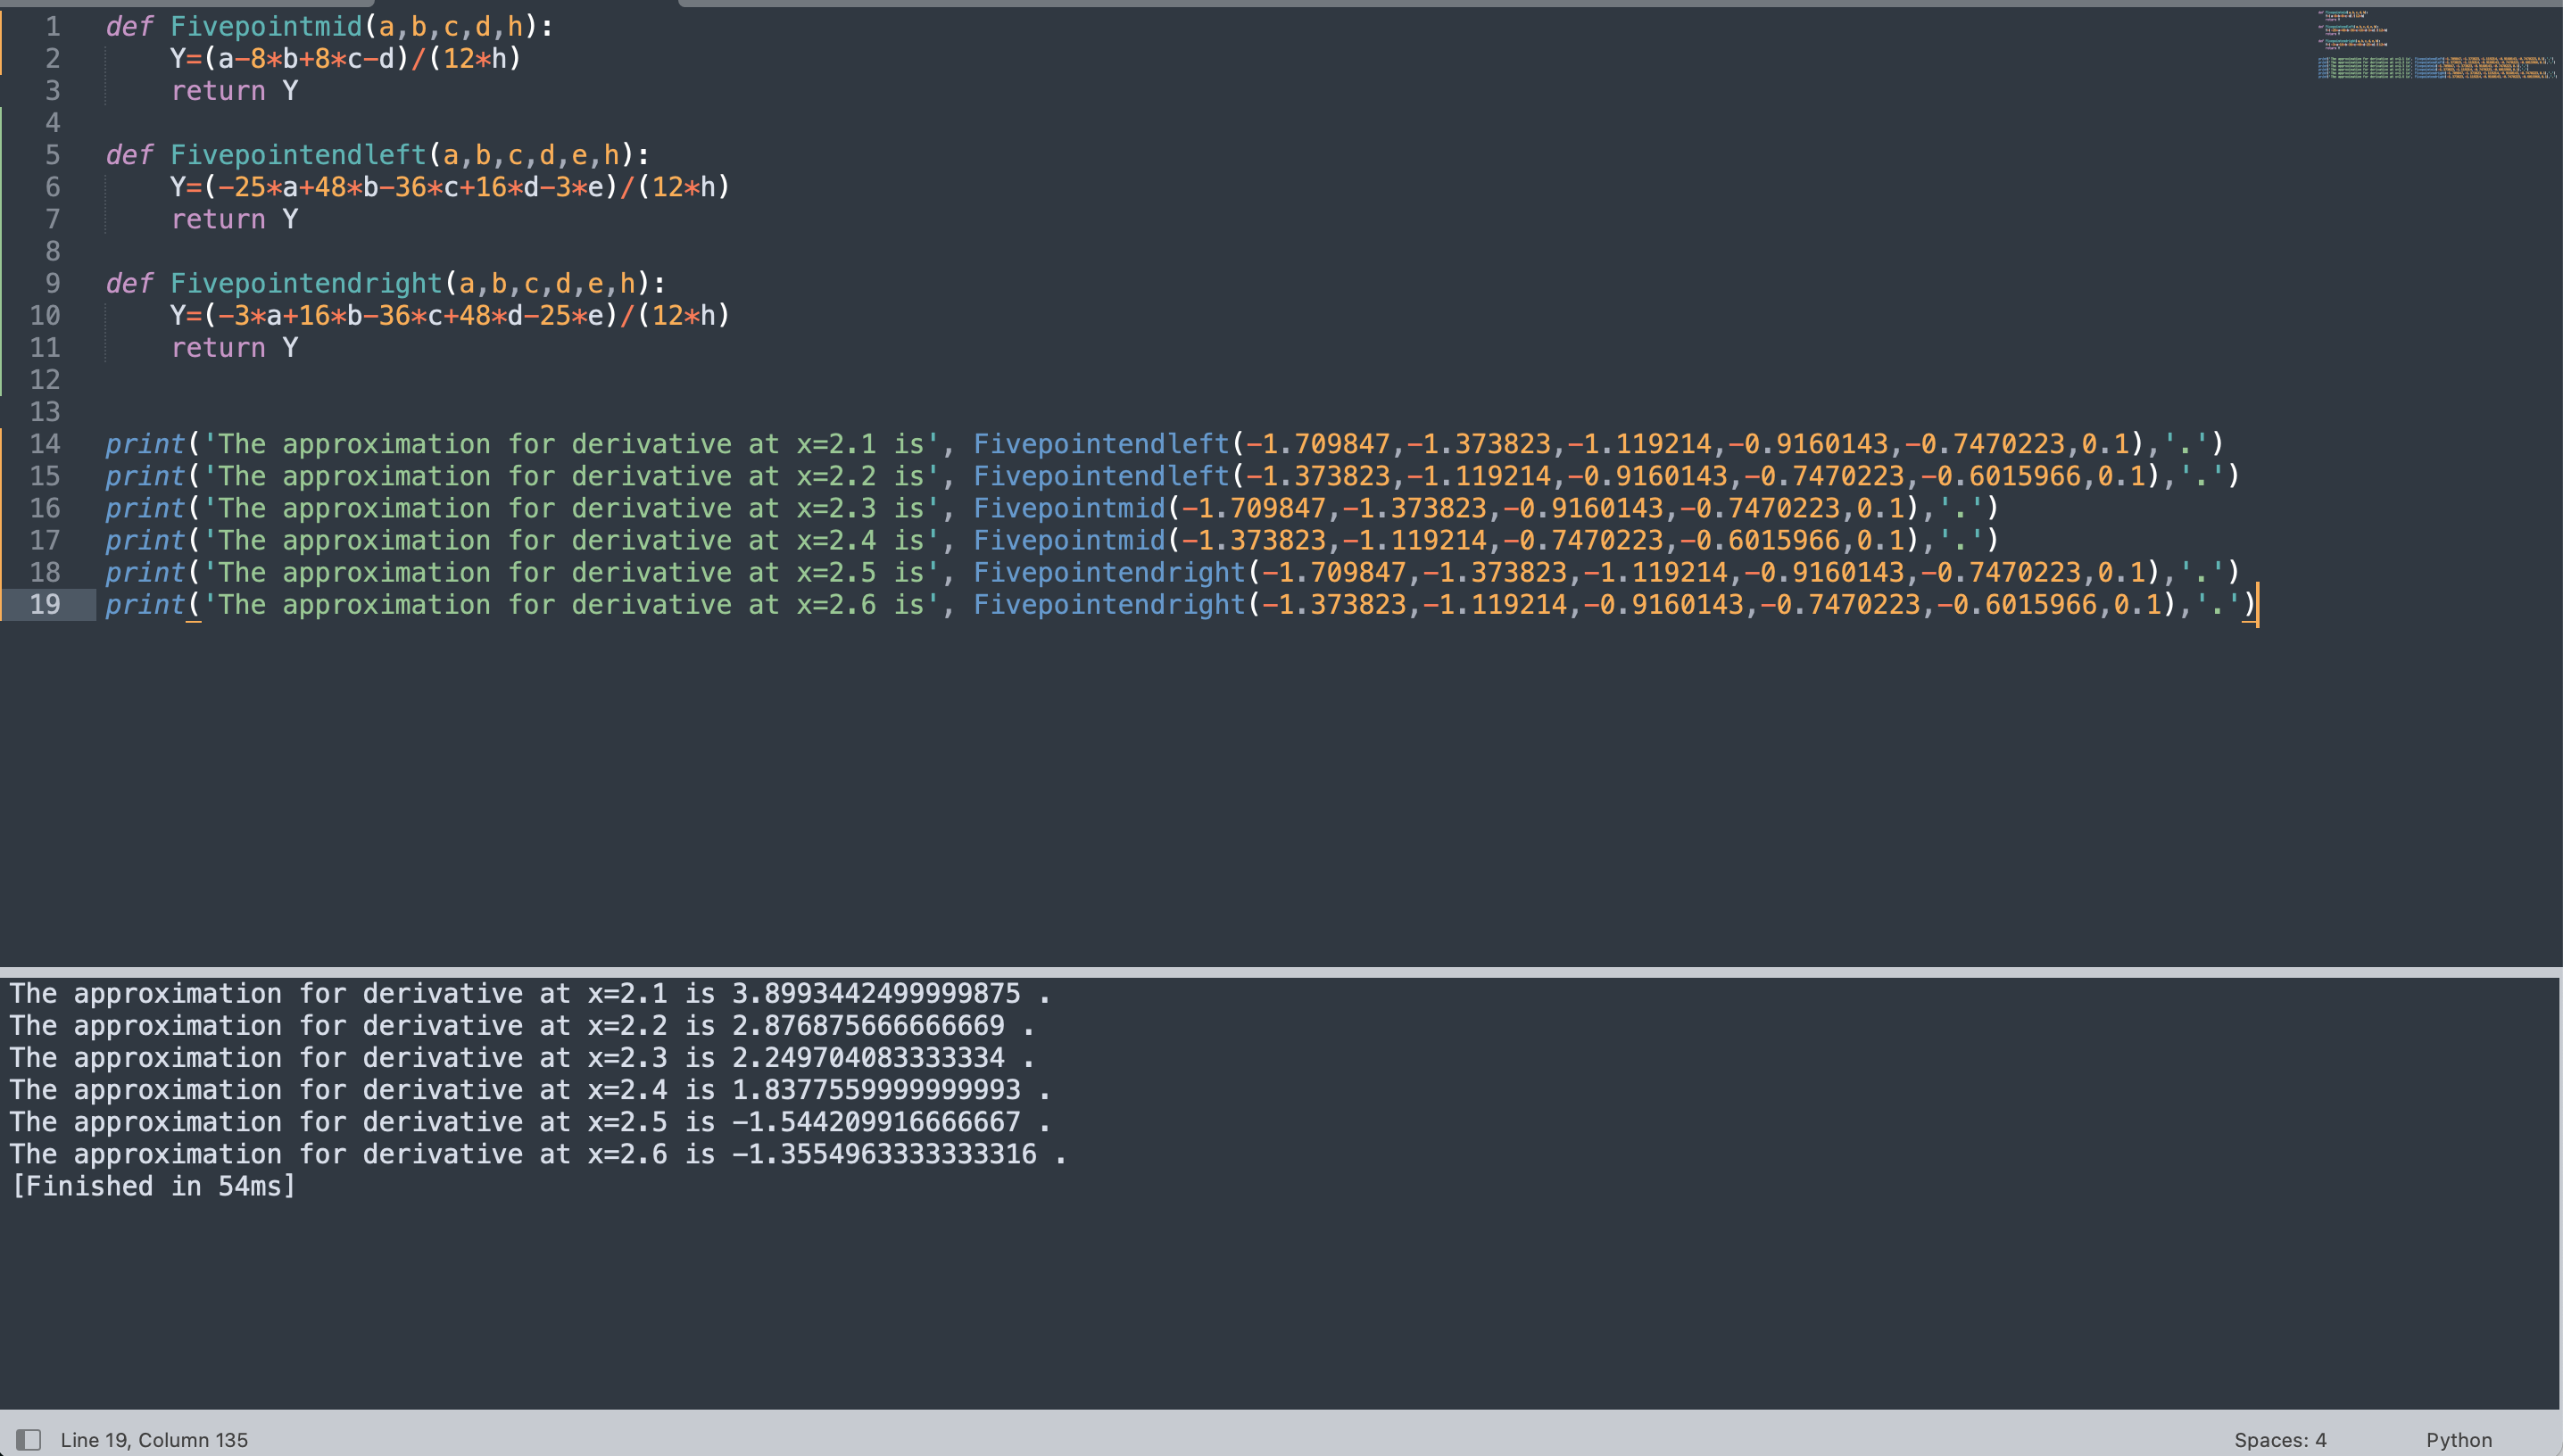
\includegraphics[scale=0.28]{Program1}
    \end{figure}

    We write down the results in the table below, where we \textbf{reserve seven significant digits} for the result.
    \begin{table}[htbp]
    \centering
    \caption{Results of 4.1/5a}
    \begin{tabular}{c|c|c|c}
    \toprule
    \textbf{x} & \textbf{$f(x)$} & \textbf{$f'(x)$} & \textbf{Applied Formulas} \\ 
    \midrule
    2.1 & -1.709847 & 3.899344 &4.1/(4.7)\\
    2.2 & -1.373823 & 2.876876 &4.1/(4.7)\\
    2.3 & -1.119214 & 2.249704 &4.1/(4.6) \\
    2.4 & -0.9160143 & 1.837756&4.1/(4.6) \\
    2.5 & -0.7470223 & 1.544210&4.1/(4.7)\\
    2.6 & -0.6015966 & 1.355496&4.1/(4.7)\\
    \bottomrule
    \end{tabular}
    \end{table}

\section{3. Application of Richardson's Extraposition (4.2/8,9)}
\subsection{3.1 Solution of 4.2/8}
    \noindent\textbf{Solution:} We have
    \begin{equation}
    f'(x_{0})=N_{1}(h)-\frac{f''(x_{0})}{2}\cdot h
    -\frac{f'''(x_{0})}{6}\cdot h^2+O(h^3),
    \end{equation}
    where $N_{1}(h)=(f(x_{0}+h)-f(x_{0}))/h$. 
    Replacing $h$ with $h/2$ gives 
    \begin{equation}
    f'(x_{0})=N_{1}(\frac{h}{2})-\frac{f''(x_{0})}{2}\cdot \frac{h}{2}
    -\frac{f'''(x_{0})}{6}\cdot \frac{h^2}{4}+O(h^3),
    \end{equation}
    Therefore subtract (1) from twice (2) gives
    \begin{equation}
    f'(x_{0})=2\cdot N_{1}(\frac{h}{2})-N_{1}(h)
    +\frac{f'''(x_{0})}{6}\cdot \frac{h^2}{2}+O(h^3),
    \end{equation}

    Similarly we can replace $h$ in (3) with $h/2$ gives 
    \begin{equation}
    f'(x_{0})=2\cdot N_{1}(\frac{h}{4})-N_{1}(\frac{h}{2})
    +\frac{f'''(x_{0})}{6}\cdot \frac{h^2}{8}+O(h^3).
    \end{equation}

    Therefore subtract (3) from four times (4) finally gives
    $$
    3\cdot f'(x_{0})=6\cdot N_{1}(\frac{h}{2})-3\cdot N_{1}(h)+O(h^3).
    $$
    And thus if we write $N_{1}(h)=(f(x_{0}+h)-f(x_{0}))/h$,
    $$N_{3}(h)=2\cdot N_{1}(\frac{h}{2})-N_{1}(h)$$
    is the formula that we want.

\subsection{3.2 Solution of 4.2/9}
\noindent\textbf{Solution:}
    We have by replacing $h$ by $h/3$
    \begin{equation}
    M=N(\frac{h}{3})+K_{1}\frac{h}{3}+K_{2}\frac{h^2}{9}+O(h^3)
    \end{equation}

    Subtracing (5) from three times the original equation in question gives  
    \begin{equation}
    2M=3N(\frac{h}{3})-N(h)-K_{2}\frac{2h^2}{3}+O(h^3)=2N_{2}(h)-K_{2}\frac{2h^2}{3}+O(h^3)
    \end{equation}

    Similarly we have 
    \begin{equation}
    2M=3N(\frac{h}{9})-N(\frac{h}{3})-K_{2}\frac{2h^2}{27}+O(h^3)=2N_{2}(\frac{h}{3})-K_{2}\frac{2h^2}{27}+O(h^3),
    \end{equation}
    and accordingly we have
    \begin{equation}
    16M=18N_{2}(\frac{h}{3})-2N_{2}(h)+O(h^3).
    \end{equation}

    Finally both equations together gives the results.
    \begin{align*}
    N_{2}(h)&=\frac{3}{2}\cdot N(\frac{h}{3})-\frac{N(h)}{2}=N(\frac{h}{3})+\frac{N(\frac{h}{3})-N(h)}{2}.\\
    N_{3}(h)&=\frac{9}{8}\cdot N_{2}(\frac{h}{3})-\frac{N_{2}(h)}{8}=N_{2}(\frac{h}{3})+\frac{N_{2}(\frac{h}{3})-N_{2}(h)}{8}.
    \end{align*}

\section{4. Application of Composite Numerical Integration (4.4/7)}
    To interpret the value of 
    $$\int_{0}^{2}e^{2x}sin(3x)dx \quad \text{(question 4.4/7)}
    $$
    by means of numerical integration. First we calculate an actual value of it as follows
    $$ \int_{0}^{2}e^{2x}sin(3x)dx=Im(\int_{0}^{2}e^{(2+3i)x}dx)=\frac{3+e^4(2sin6-3cos6)}{13}\approx -14.2139771298625\ldots
    $$
    Let $f(x):=e^{2x}sin(3x)$, we have $f''(x)=12cos(3x)e^{2x}-5sin(3x)e^{2x}$ and 
    $$ max\{|f''(x)|:x\in[0,2]\}=|f''(2)|=e^4(12cos6-5sin6)\approx705.360102876099\ldots
    $$

    Therefore for \textbf{composite trapezoidal rule}, \textbf{the error form} is 
    $$ |\frac{b-a}{12}h^2f''(\xi)|\leq |\frac{f''(2)}{6}h^2|<10^{-4}\implies h<\big(\frac{6\cdot 10^{-4}}{f''(2)}\big)^{1/2}=0.000922295691056397\ldots
    $$
    and thus 
    $$ n\geq \frac{2}{0.000922295691056397}=2168.5 \implies n\geq 2169.
    $$

    Similarly for \textbf{composite simpsons rule} we have
    $$ |\frac{b-a}{180}h^4f^{(4)}(\xi)|<10^{-4}
    \implies h<0.037658\ldots \text{ and } n\geq 54.
    $$

    And \textbf{composite midpoint rule} we have
    $$ |\frac{b-a}{6}h^2f''(\xi)|\leq |\frac{f''(2)}{6}h^2|<10^{-4}\implies h<0.00065216\ldots \text{ and } n\geq 3067.
    $$

    Finally we have 
    \begin{table}[htbp]
    \centering
    \caption{Results of 4.4/7}
    \begin{tabular}{c|c|c}
    \toprule
    \textbf{Applied Methods} & \textbf{Maximum Value of h} & \textbf{Minimum Value of n} \\ 
    \midrule
    composite trapezoidal rule & 0.000922295691 & 2169 \\
    composite simpsons rule & 0.037658 & 54 \\
    composite midpoint rule &  0.00065216 & 3067 \\
    \bottomrule
    \end{tabular}
    \end{table}

    and for completeness we give the approximation 
    \begin{table}[htbp]
    \centering
    \caption{Results of 4.4/7}
    \begin{tabular}{c|c|c|c}
    \toprule
    \textbf{Applied Methods} & \textbf{n} & \textbf{Approximation Value } & \textbf{Error}\\ 
    \midrule
    composite trapezoidal rule & 2169 & -14.213968361108893 &-8.768753627208525e-06 \\
    composite simpsons rule & 54  &-14.213964900134542 &-1.2229727978763094e-05\\
    composite midpoint rule &  3067  &-14.21065207837095 &-0.0033250514915703633\\ 
    \bottomrule
    \end{tabular}
    \end{table}

    For completeness, we write down the codes and run the program for each case, e.g. n=2169 with composite trapezoidal rule.

    \begin{figure}[h]
    \centering
    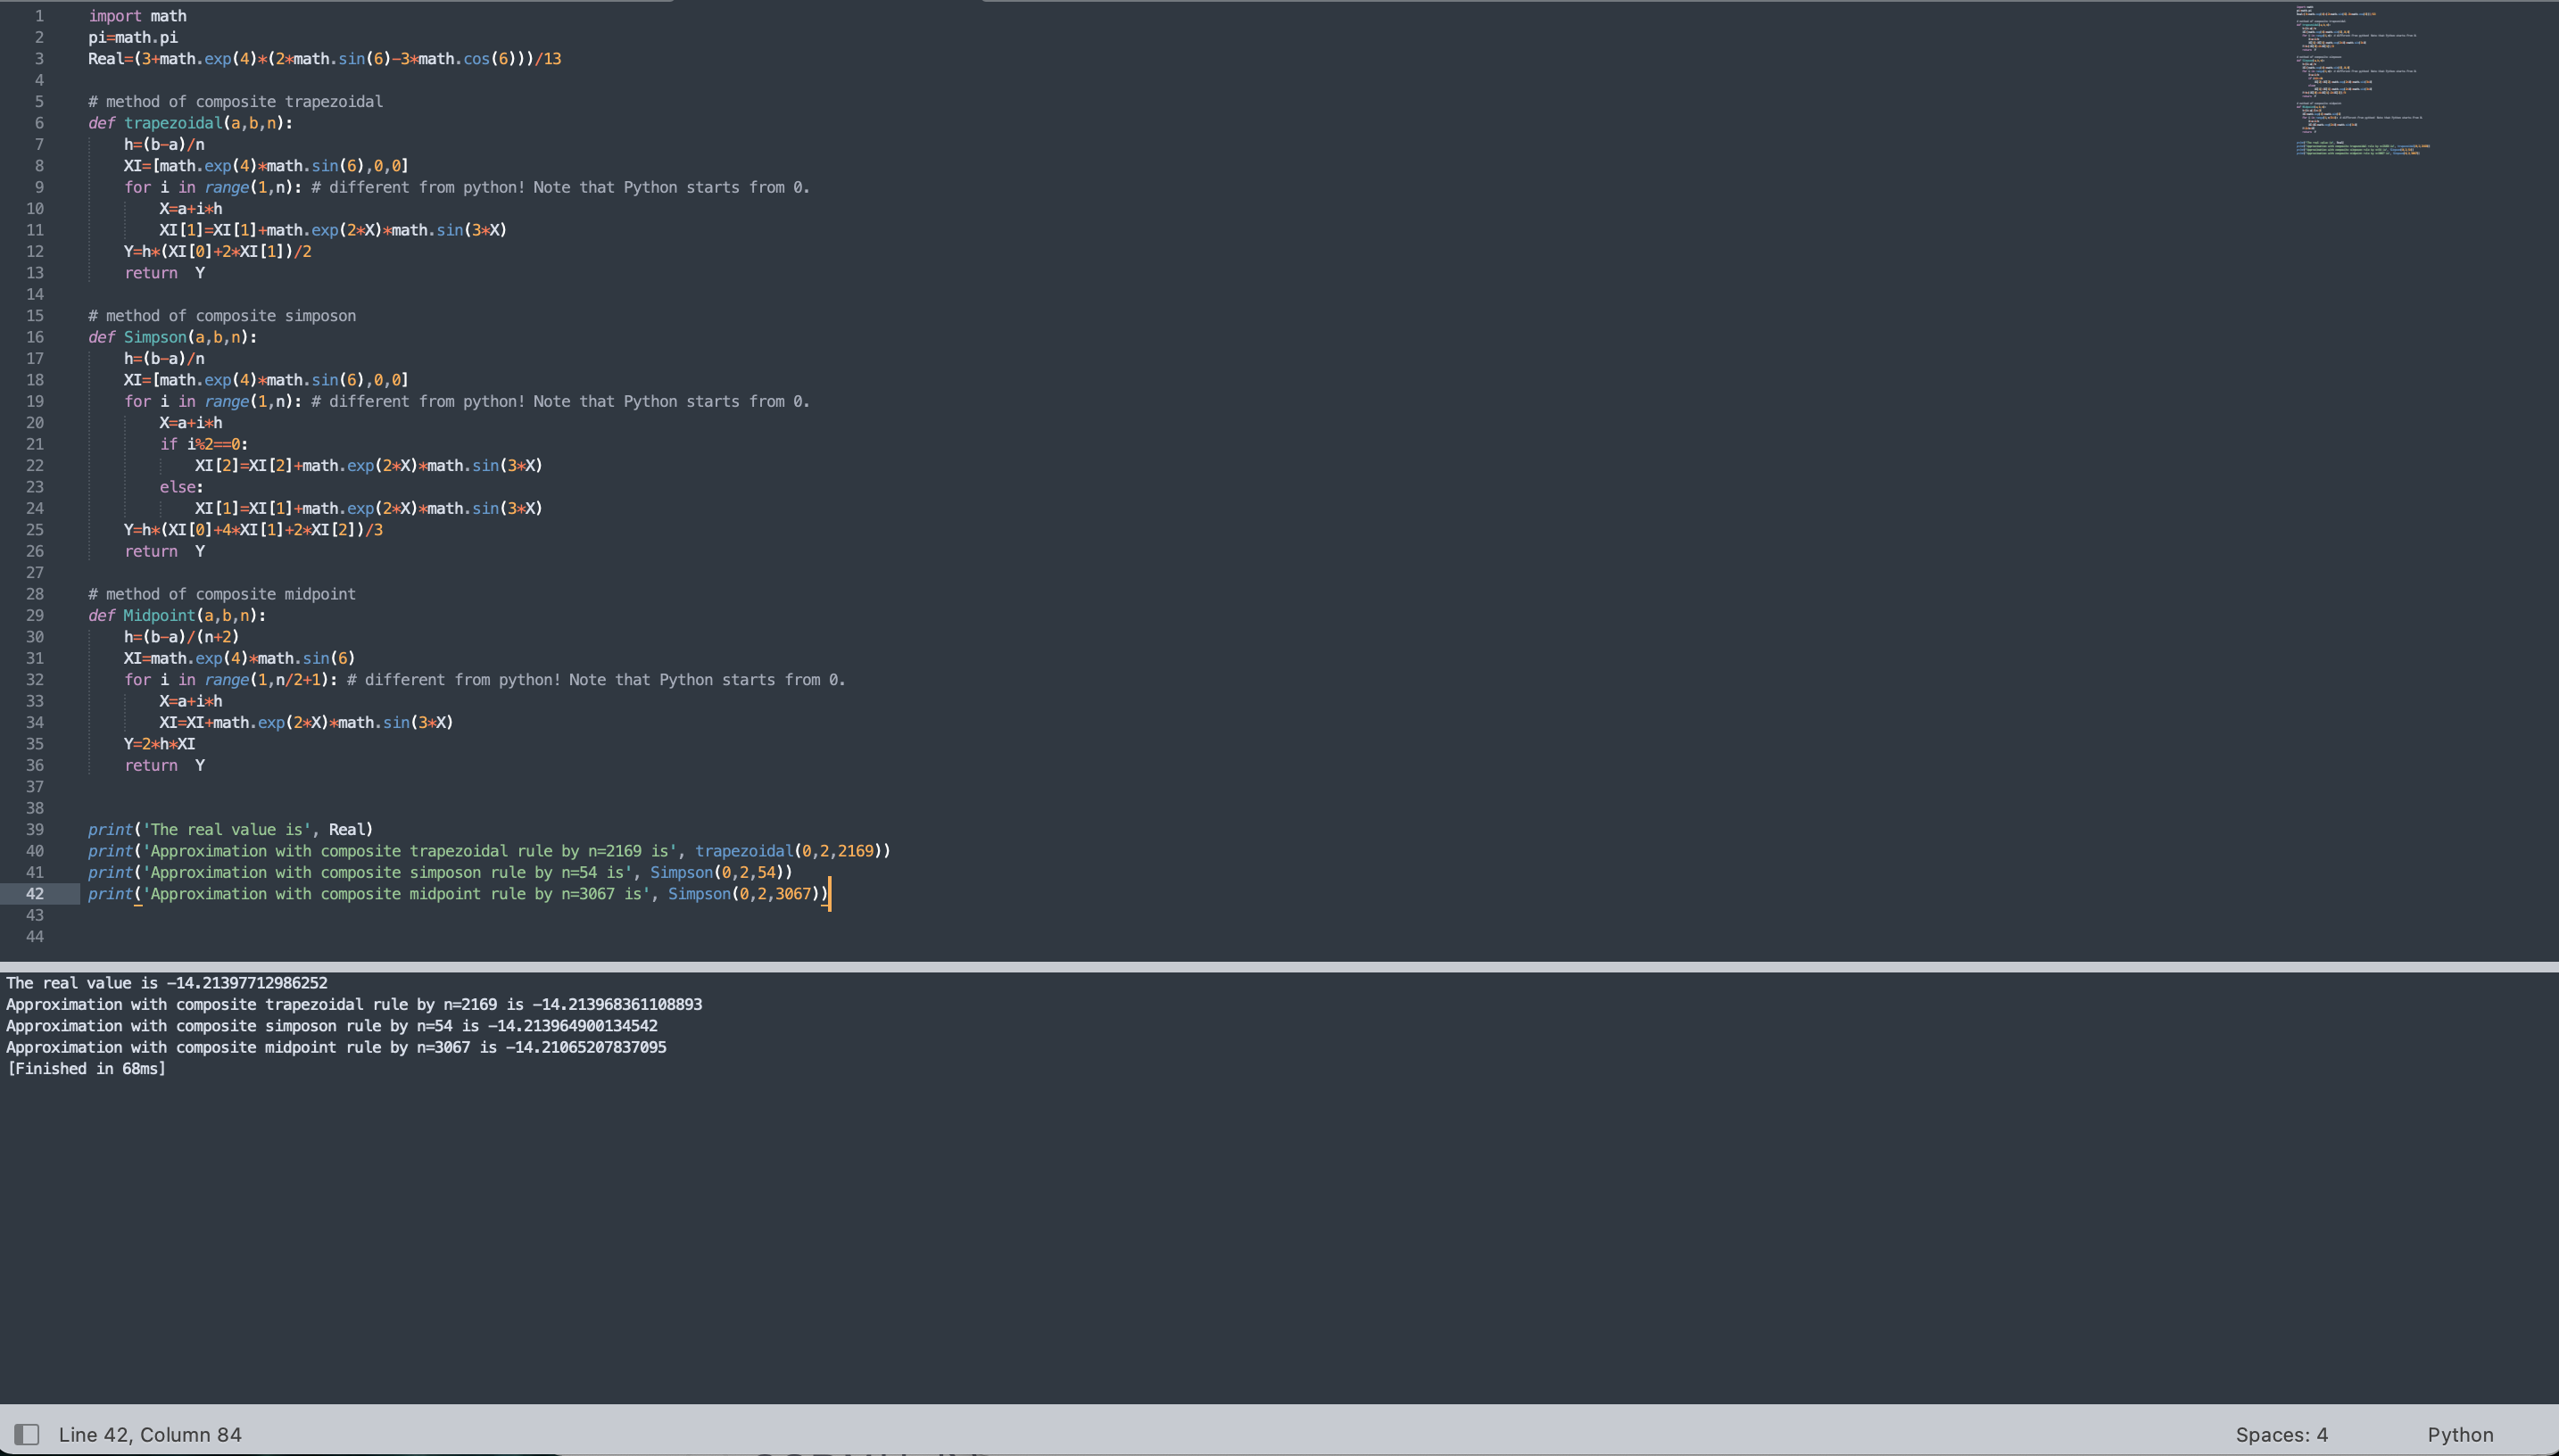
\includegraphics[scale=0.3]{Program2}
    \end{figure}

\newpage

\section{5. Application of Romberg Integration (4.5/4b)}
    
    4.5/4b requires approximation of $\int_{0}^{0.3}f(x)dx$ where
    $$
    f(X)=\left\{
    \begin{array}{rcl}
    &X^3+1  & {0 \leq X\leq 0.1 }\\
    &1.001+0.03(X-0.1)+0.3(X-0.1)^2+2(X-0.1)^3 & {0.1 < X\leq 0.2 }\\
    &1.009+0.15(X-0.2)+0.15(X-0.2)^2+0.9(X-0.2)^3  & {0.2 < X\leq 0.3 }\\
    \end{array} \right.
    $$

    And we run the program as follows. (Meanwhile we display the running time.)

    \begin{figure}[h]
    \centering
    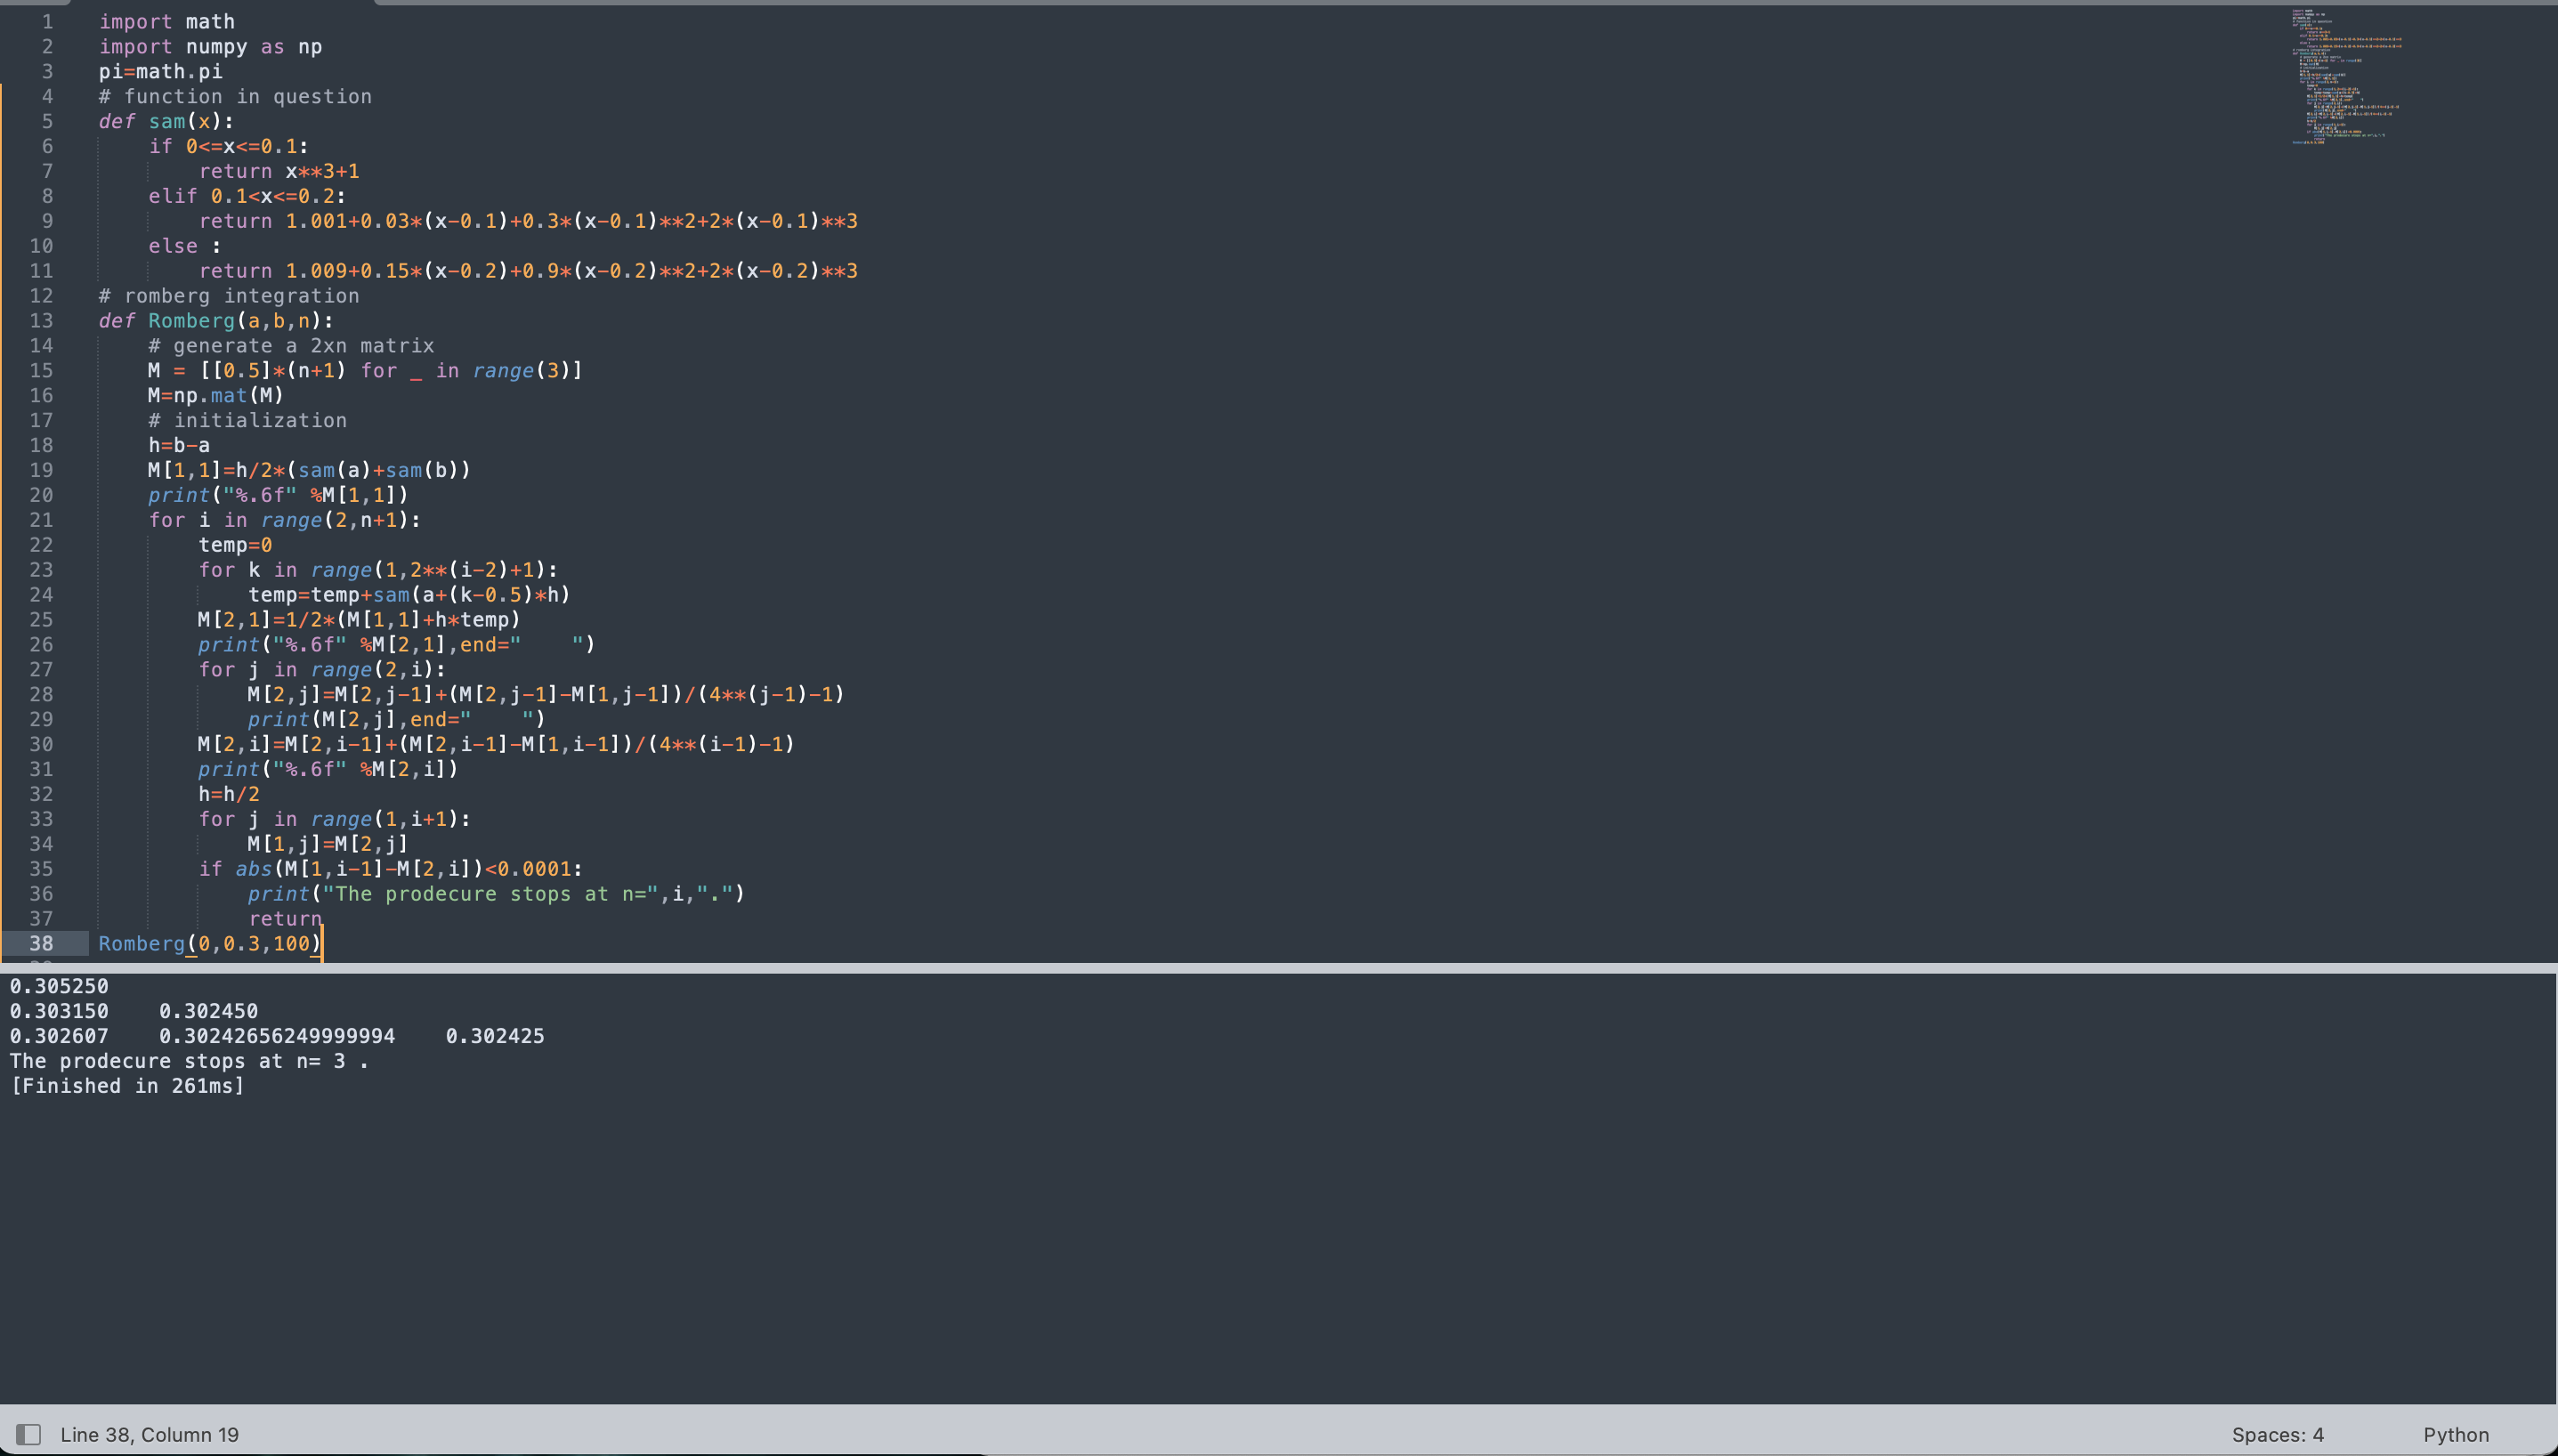
\includegraphics[scale=0.28]{Program3}
    \end{figure}

    The real value is 
    $$\int_{0}^{0.3}f(x)dx=(\int_{0}^{0.1}+\int_{0.1}^{0.2}+\int_{0.2}^{0.3})f(x)dx=0.100025+0.10031+0.102=0.30256
    $$

    We show the generated results in a table just as table 4.9. Note: we end at n=3 since $R_{n-1,n-1}$ and $R_{n,n}$ agree to within $10^{-4}$

    \begin{table}[htbp]
    \centering
    \caption{Results of 4.5/4b}
    \begin{tabular}{ccc}
    \toprule
    0.305250 & 0 & 0 \\
    0.303150 & 0.302450 & 0 \\
    0.302607 & 0.30242656249999994 & 0.302425 \\ 
    \bottomrule
    \end{tabular}
    \end{table}

    We see that the best approximation is given by (either one)

    $$\int_{0}^{0.3}f(x)dx-R_{31}=0.30256-0.302607=-4.7\times 10^{-5}
    $$
    $$\int_{0}^{0.3}f(x)dx-R_{32}=0.30256-0.30242656249999994=1.3\times 10^{-4}
    $$
    $$\int_{0}^{0.3}f(x)dx-R_{33}=0.30256-0.302425=1.3\times 10^{-4}
    $$

    We see that the romberg technique has two desirable features:

    1.It allows an entire new row easily calculated from above.

    2.It uses an averaging technique to produce formulas with higher-order tuncation error.

\newpage
\section{6. Application of Gaussian Quadrature (4.7/1b)}
    The question is to determine values of $\int_{0}^{1}x^2e^{-x}dx$ with 2/3/4/5-point Gaussian Quadrature. 

    First the real value is 
    $$\int_{0}^{1}x^2e^{-x}dx=-e^{-1}-\int_{0}^{1}2xd(e^{-x})=2-\frac{5}{e}=0.160602794142788\ldots
    $$

    Using 4.7/(4.42) we have
    $$ \int_{0}^{1}f(x)dx=\int_{-1}^{1}f(\frac{t+1}{2})\cdot\frac{1}{2}dt
    $$

    where $f(x):=x^2e^{-x}$ and we let $g(x):=f(\frac{t+1}{2})\cdot\frac{1}{2}$. Using values in table 4.11 we write down and codes and run the program as follows. (Meanwhile we display the running time.)

    \begin{figure}[h]
    \centering
    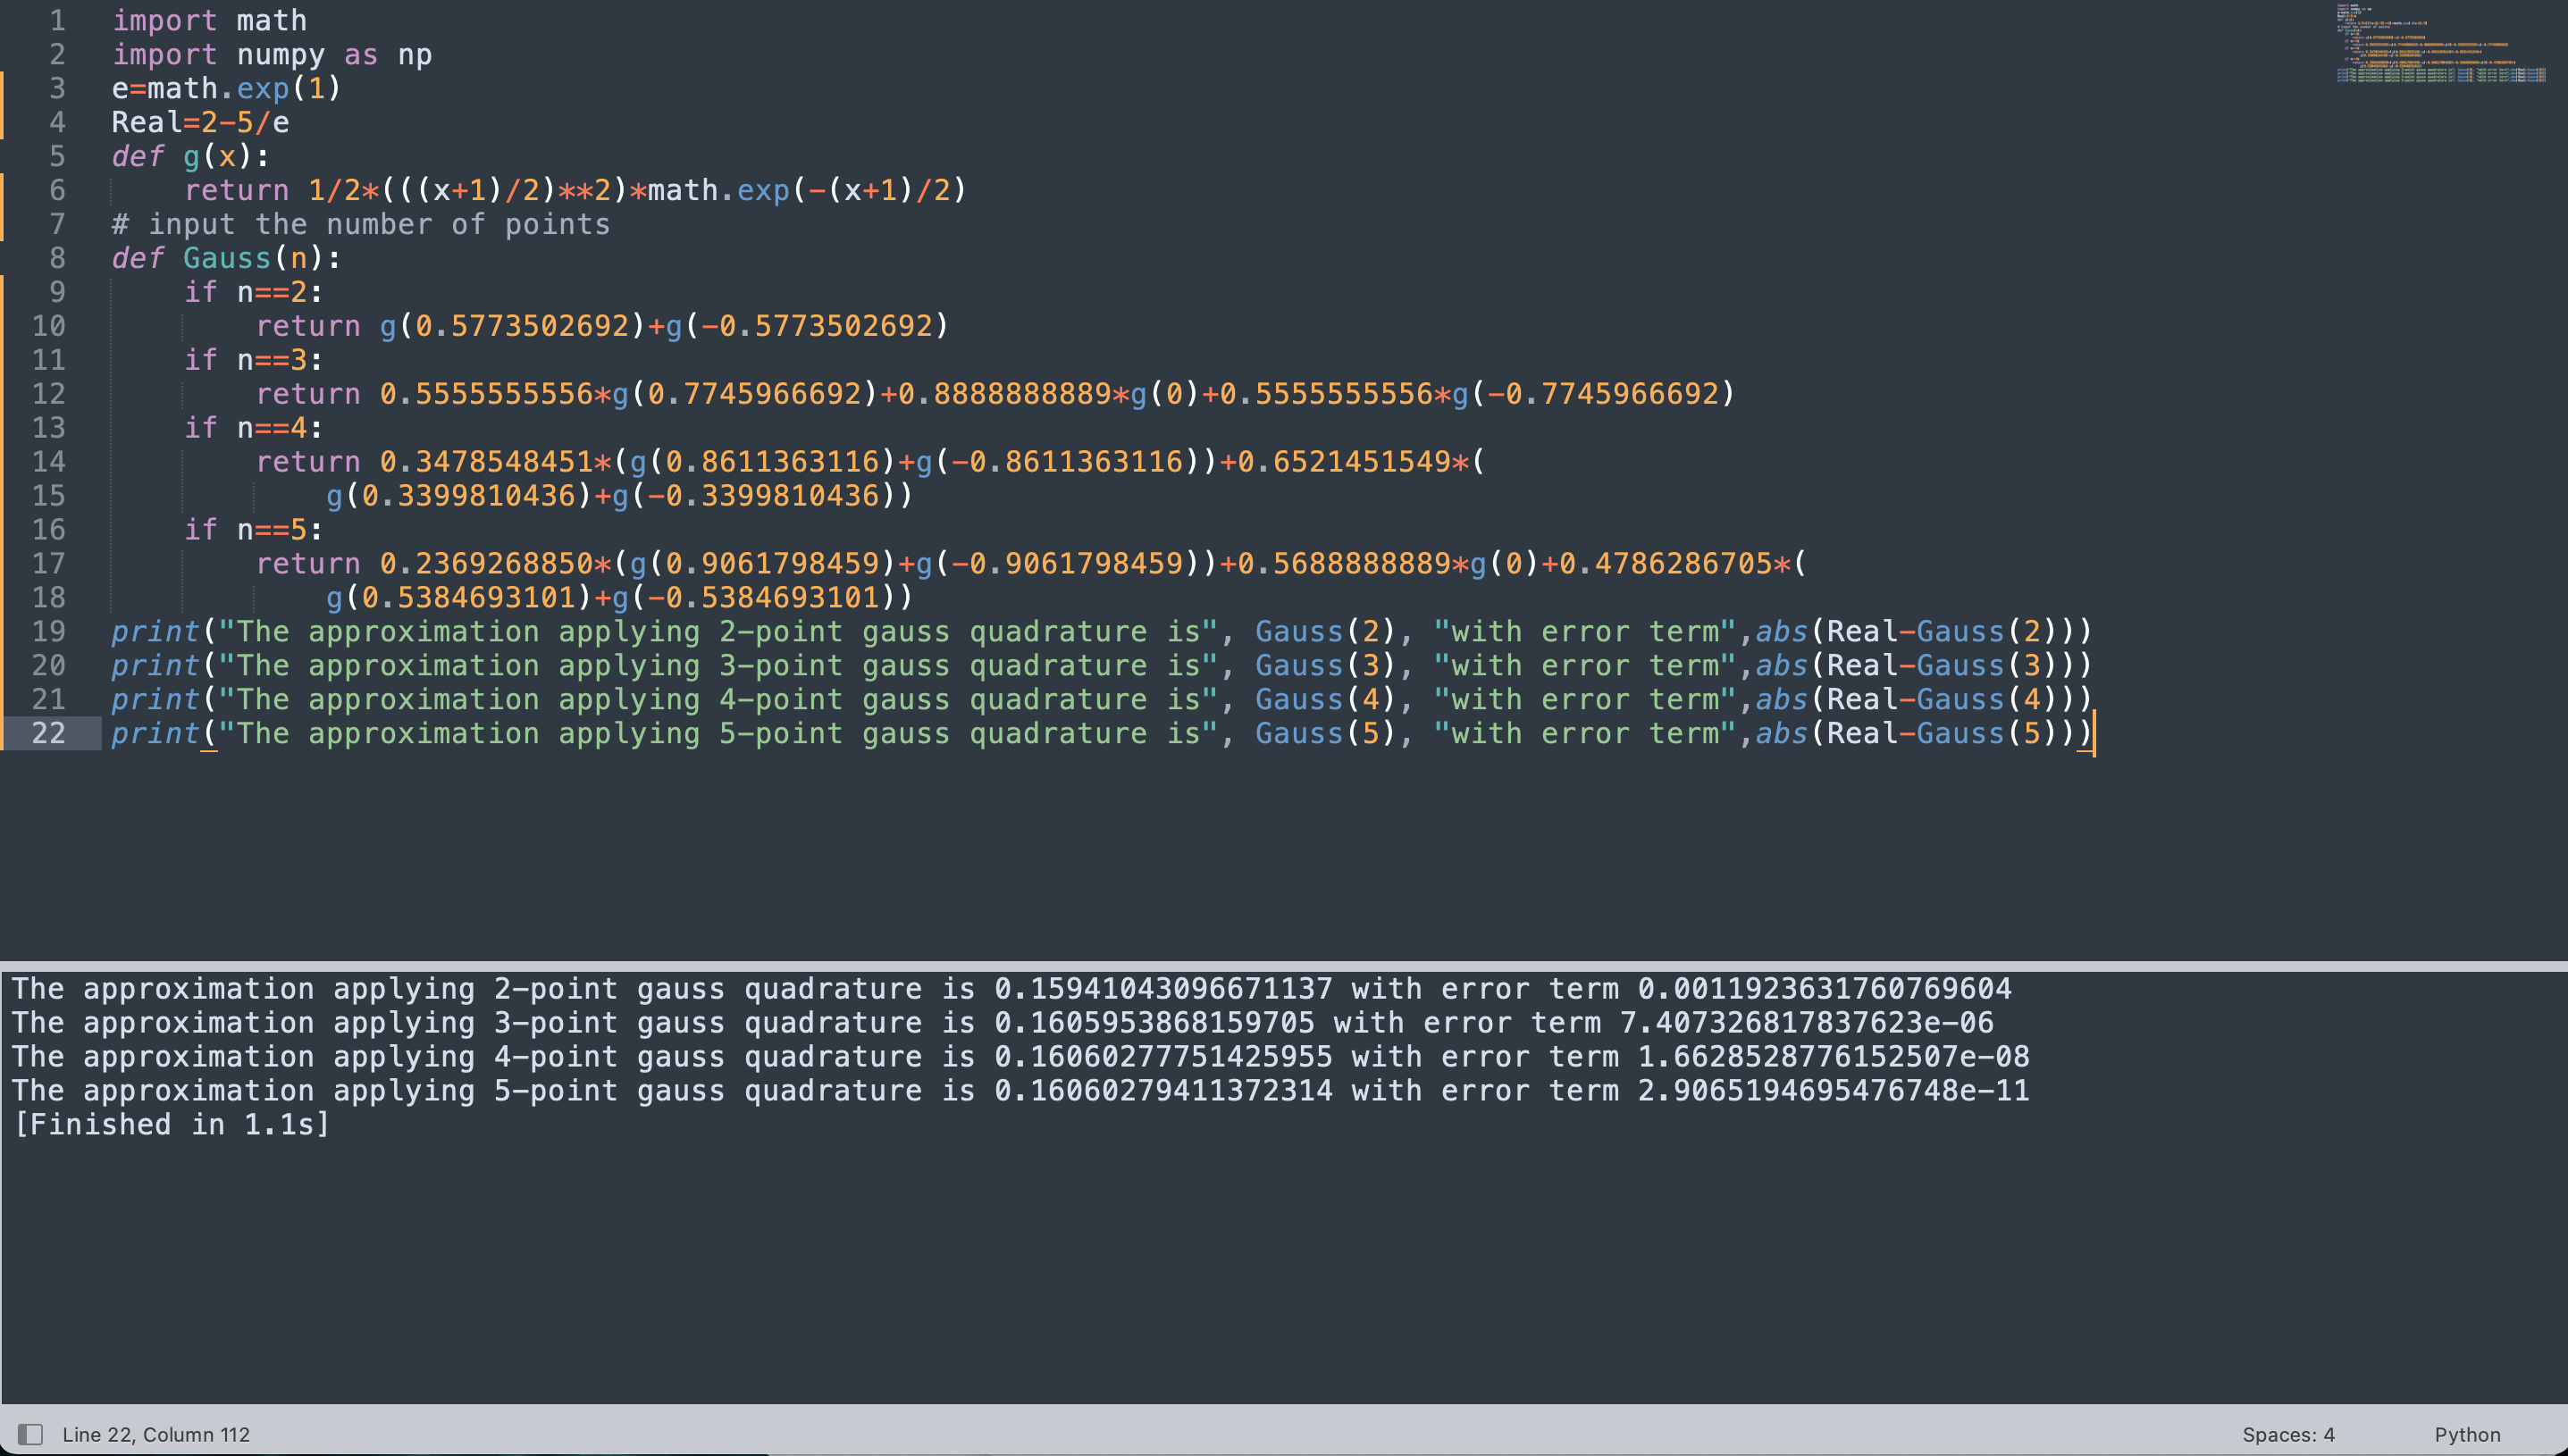
\includegraphics[scale=0.3]{Program4}
    \end{figure}

    The program give the following gaussian quadrature approximations for the problem:

    \begin{align*}
    \text{n=2: } \int_{0}^{1}f(x)dx=&g(0.5773502692)+g(-0.5773502692)=0.15941043096671137 \\
    \text{n=3: } \int_{0}^{1}f(x)dx=&0.5555555556\cdot \bigg[g(0.7745966692)+g(-0.7745966692)\bigg]+0.8888888889\cdot g(0)\\
    =&0.1605953868159705\\
    \text{n=4: } \int_{0}^{1}f(x)dx=&0.3478548451\cdot \bigg[g(0.8611363116)+g(-0.8611363116)\bigg]\\
    &+0.6521451549\cdot \bigg[g(0.3399810436)+g(-0.3399810436)\bigg] \\
    =&0.16060277751425955
    \end{align*}

    and

    \begin{align*}
    \text{n=5: } \int_{0}^{1}f(x)dx=&0.2369268850\cdot\bigg[g(0.9061798459)+g(-0.9061798459)\bigg]+0.5688888889\cdot g(0)\\
    &+0.4786286705\cdot \bigg[g(0.5384693101)+g(-0.5384693101)\bigg] \\
    =&0.16060279411372314
    \end{align*}

    where $g(x):=f(\frac{t+1}{2})\cdot \frac{1}{2}$.

    And therefore a table for results 

    \begin{table}[htbp]
    \centering
    \caption{Results of 4.7/1b}
    \begin{tabular}{c|c|c}
    \toprule
    \textbf{Applied Methods} & \textbf{Approximation Value } & \textbf{Error}\\ 
    \midrule
    2-point Gaussian Quadrature & 0.15941043096671137 &$1.1923631760769604\times 10^{-3}$ \\
    3-point Gaussian Quadrature & 0.1605953868159705 &$7.407326817837623\times 10^{-6}$\\
    4-point Gaussian Quadrature &  0.16060277751425955 &$1.6628528776152507\times 10^{-8}$\\ 
    5-point Gaussian Quadrature &  0.16060279411372314  &$2.9065194695476748\times 10^{-11}$\\ 
    \bottomrule
    \end{tabular}
    \end{table}

    which shows that the more nodes involves, the more accurate the results approximate the real value.

\section{7. Double Integration (4.8/1b)}
    To approximate 
    $$\int_{0}^{0.5}\int_{0}^{0.5}e^{y-x}dxdy \text{(4.8/1b),}$$ 
    we have simpson's double integration (n=m=4) and gaussian double integration (n=m=3). Using values in table 4.11 we write down and codes and run the program as follows. (Meanwhile we display the running time.)

    \begin{figure}[h]
    \centering
    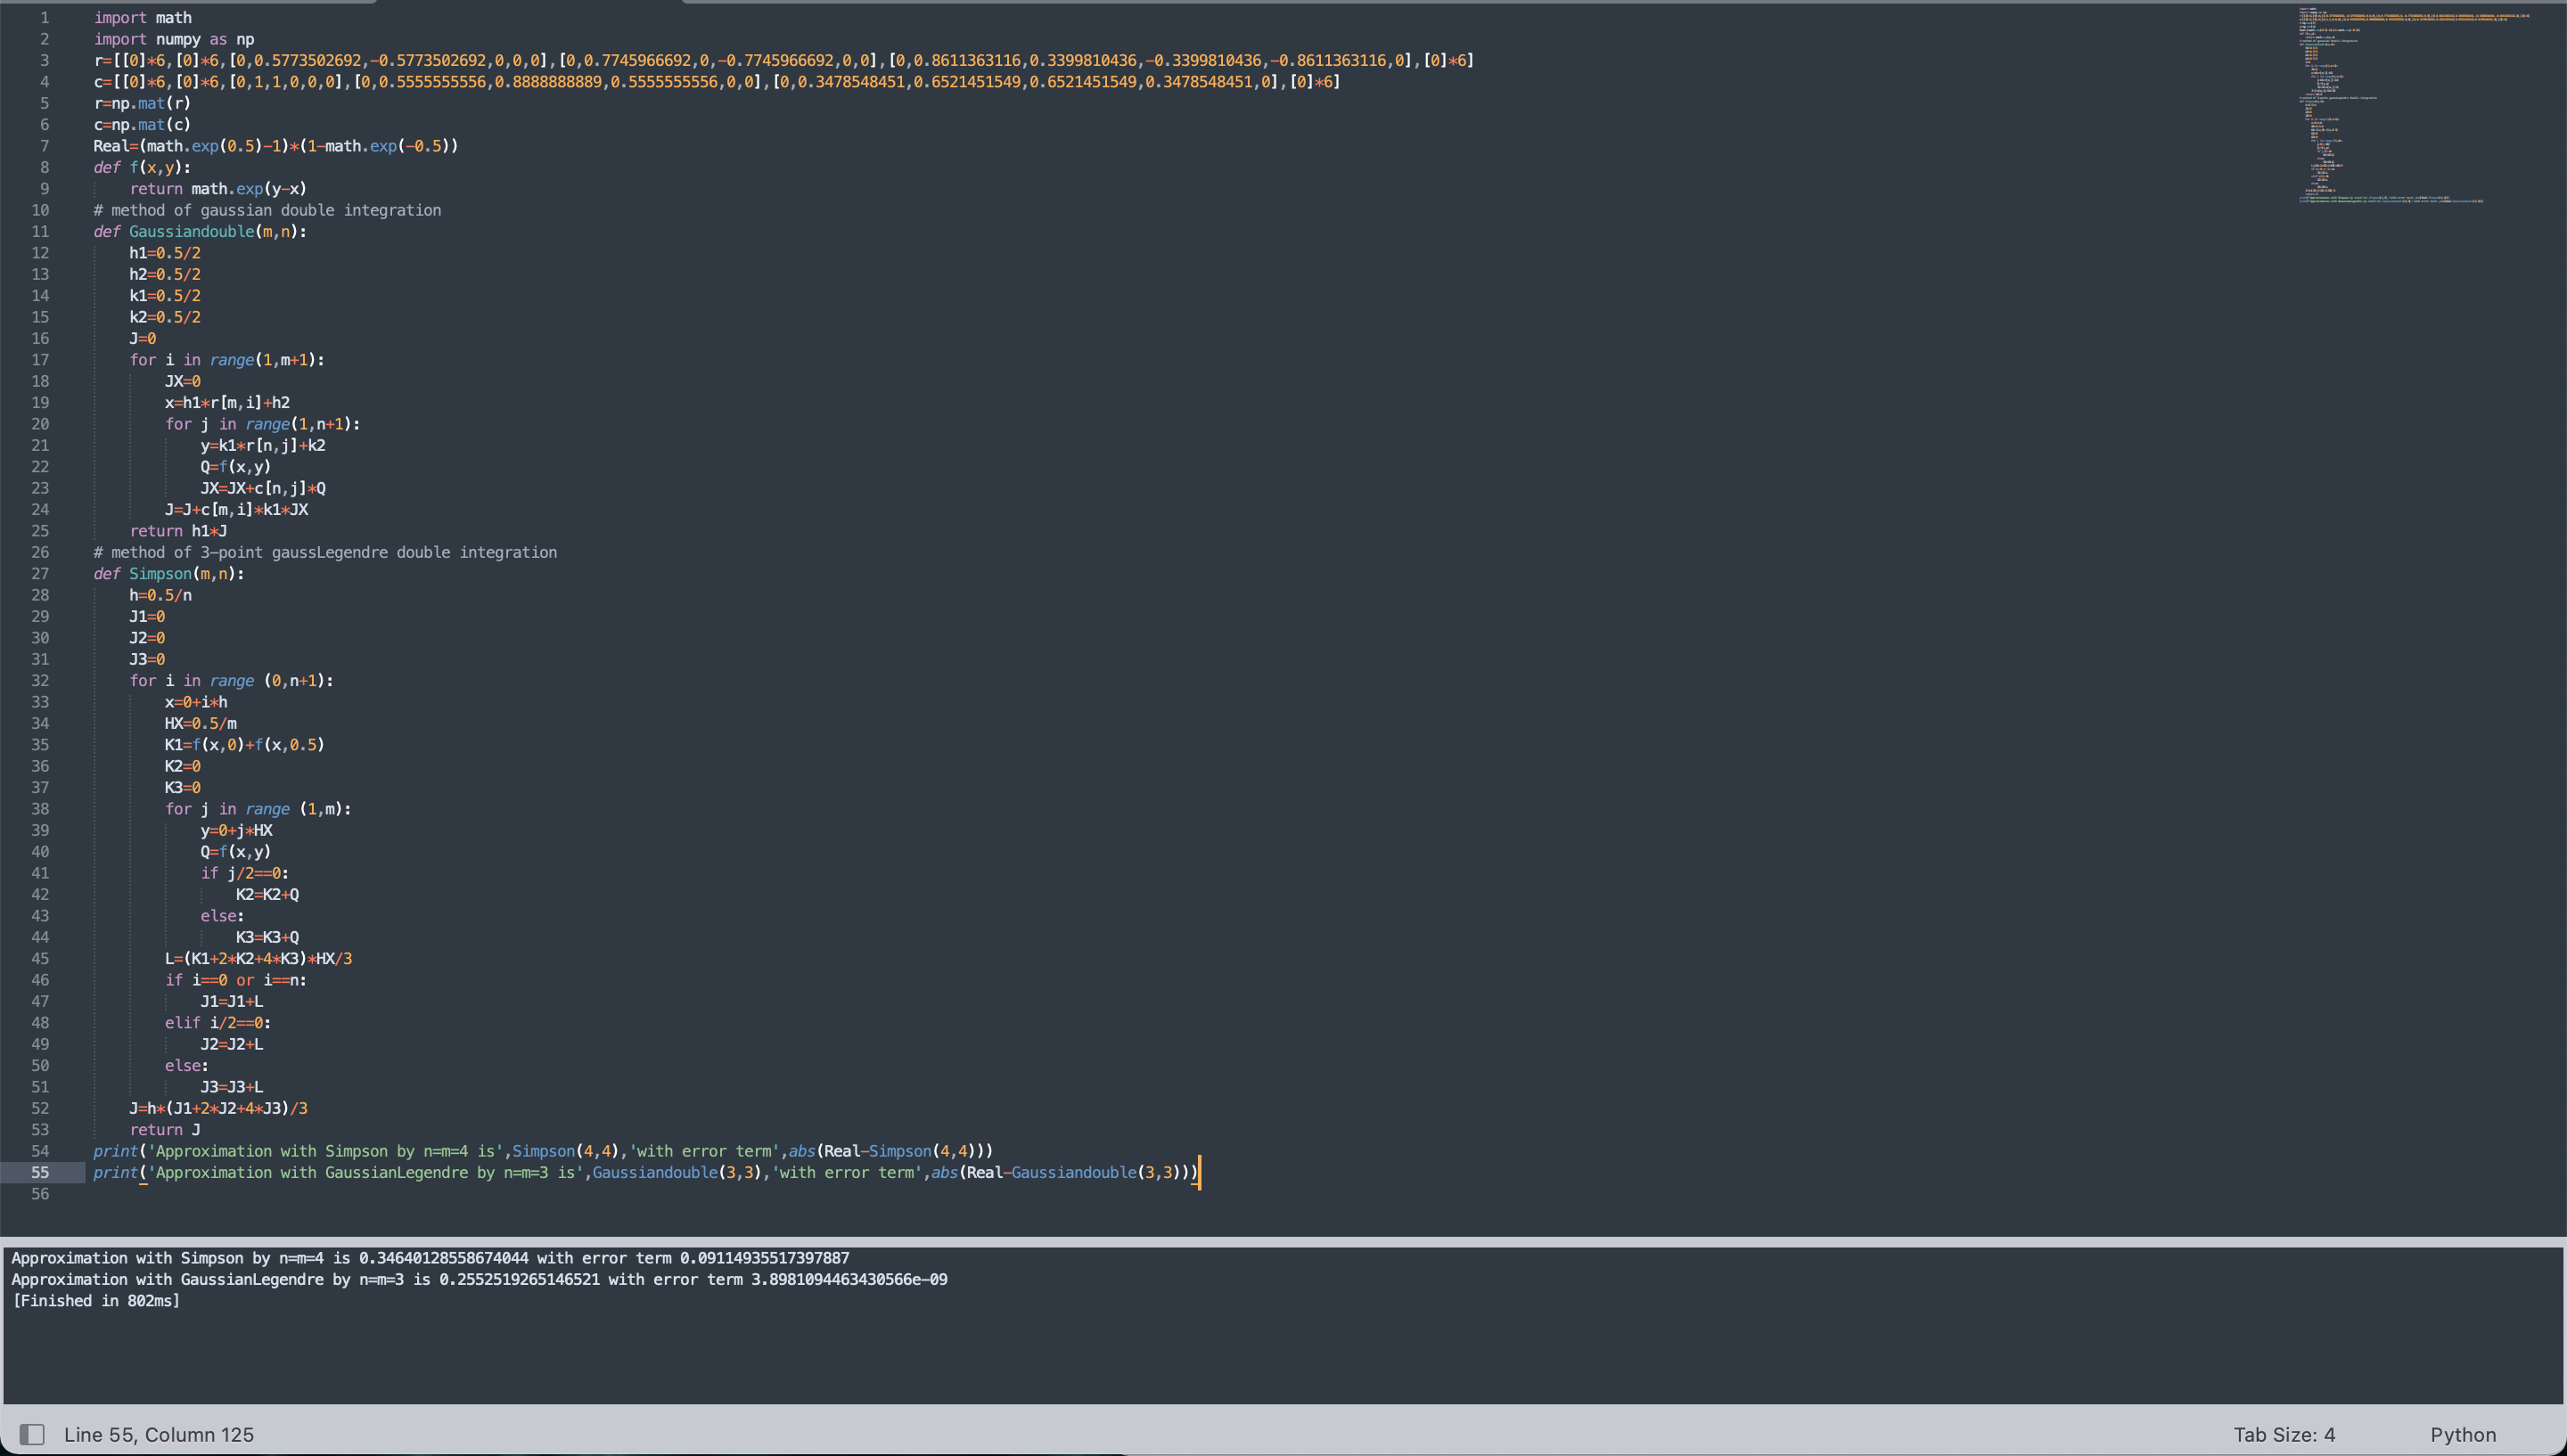
\includegraphics[scale=0.3]{Program5}
    \end{figure}

    And therefore a table for results above. 

    \begin{table}[htbp]
    \centering
    \caption{Results of 4.8/1b}
    \begin{tabular}{c|c|c}
    \toprule
    \textbf{Applied Methods} & \textbf{Approximation Value } & \textbf{Error}\\ 
    \midrule
    Simpson's rule (n=m=4)& 0.34640128558674044 &$9.114935517397887 \times 10^{-2}$\\
    GaussianLegendre (n=m=3)&0.2552519265146521& $3.8981094463430566\times 10^{-9}$\\
    \bottomrule
    \end{tabular}
    \end{table}

    We see that the gaussian double inetegration involves fewer functional evaluations (9 functional evaluations) compared with 16 functional evaluations of Simpson's rule. Moreover, the gaussian double inetegration acquires itself higher-order tuncation error. Thus the result is accurate to within $3.9\times 10^{-9}$ compared to the accuracy $9\times 10^{-2}$ of Simpson's rule.

\section{4. Code Appendix}
    \subsection{4.1 Five-point Fomulas}
    \begin{python}
    # method of five-point midpoint(endpoint) formula
    # midpoint version
    def Fivepointmid(a,b,c,d,h):
        Y=(a-8*b+8*c-d)/(12*h)
        return Y
    # left endpoint version
    def Fivepointendleft(a,b,c,d,e,h):
        Y=(-25*a+48*b-36*c+16*d-3*e)/(12*h)
        return Y
    # right endpoint version
    def Fivepointendright(a,b,c,d,e,h):
        Y=(-3*a+16*b-36*c+48*d-25*e)/(12*h)
        return Y


    print('The approximation for derivative at x=2.1 is', Fivepointendleft(-1.709847,
    -1.373823,-1.119214,-0.9160143,-0.7470223,0.1),'.')
    print('The approximation for derivative at x=2.2 is', Fivepointendleft(-1.373823,
    -1.119214,-0.9160143,-0.7470223,-0.6015966,0.1),'.')
    print('The approximation for derivative at x=2.3 is', Fivepointmid(-1.709847,
    -1.373823,-0.9160143,-0.7470223,0.1),'.')
    print('The approximation for derivative at x=2.4 is', Fivepointmid(-1.373823,
    -1.119214,-0.7470223,-0.6015966,0.1),'.')
    print('The approximation for derivative at x=2.5 is', Fivepointendright(-1.709847,
    -1.373823,-1.119214,-0.9160143,-0.7470223,0.1),'.')
    print('The approximation for derivative at x=2.6 is', Fivepointendright(-1.373823,
    -1.119214,-0.9160143,-0.7470223,-0.6015966,0.1),'.')
    \end{python}

    \subsection{4.2 Composite Trapezoidal/Simposon/Midpoint Rule}
    \begin{python}
    import math
    pi=math.pi
    Real=(3+math.exp(4)*(2*math.sin(6)-3*math.cos(6)))/13  

    # method of composite trapezoidal
    def trapezoidal(a,b,n):
        h=(b-a)/n
        XI=[math.exp(4)*math.sin(6),0,0]
        for i in range(1,n): # different from python! Note that Python starts from 0.
            X=a+i*h
            XI[1]=XI[1]+math.exp(2*X)*math.sin(3*X)
        Y=h*(XI[0]+2*XI[1])/2
        return  Y

    # method of composite simposon
    def Simpson(a,b,n):
        h=(b-a)/n
        XI=[math.exp(4)*math.sin(6),0,0]
        for i in range(1,n): # different from python! Note that Python starts from 0.
            X=a+i*h
            if i%2==0:
                XI[2]=XI[2]+math.exp(2*X)*math.sin(3*X)
            else:
                XI[1]=XI[1]+math.exp(2*X)*math.sin(3*X)
        Y=h*(XI[0]+4*XI[1]+2*XI[2])/3
        return  Y

    # method of composite midpoint
    def Midpoint(a,b,n):
        h=(b-a)/(n+2)
        XI=math.exp(4)*math.sin(6)
        for i in range(1,n/2+1): # different from python! Note that Python starts from 0.
            X=a+i*h
            XI=XI+math.exp(2*X)*math.sin(3*X)
        Y=2*h*XI
        return  Y


    print('The real value is', Real)
    print('Approximation with composite trapezoidal rule by n=2168 is', trapezoidal(0,2,2168))
    print('Approximation with composite simposon rule by n=54 is', Simpson(0,2,54))
    print('Approximation with composite midpoint rule by n=3066 is', Simpson(0,2,3066))
    \end{python}

    \subsection{4.3 Romberg Integration}
    \begin{python}
    import math
    import numpy as np
    import sympy
    pi=math.pi

    def sam(x):
        if 0<=x<=0.1:
            return x**3+1
        elif 0.1<x<=0.2:
            return 1.001+0.03*(x-0.1)+0.3*(x-0.1)**2+2*(x-0.1)**3
        else :
            return 1.009+0.15*(x-0.2)+0.9*(x-0.2)**2+2*(x-0.2)**3

    def Romberg(a,b,n):
        # generate a 2xn matrix 
        M = [[0.5]*(n+1) for _ in range(3)]
        M=np.mat(M)
        # initialization
        h=b-a
        M[1,1]=h/2*(sam(a)+sam(b))
        print("%.6f" %M[1,1])
        for i in range(2,n+1):
            temp=0
            for k in range(1,2**(i-2)+1):
                temp=temp+sam(a+(k-0.5)*h)
            M[2,1]=1/2*(M[1,1]+h*temp)
            print("%.6f" %M[2,1],end="    ")
            for j in range(2,i):
                M[2,j]=M[2,j-1]+(M[2,j-1]-M[1,j-1])/(4**(j-1)-1)
                print(M[2,j],end="    ")
            M[2,i]=M[2,i-1]+(M[2,i-1]-M[1,i-1])/(4**(i-1)-1)
            print("%.6f" %M[2,i])
            h=h/2
            for j in range(1,i+1):
                M[1,j]=M[2,j]
            if abs(M[1,i-1]-M[2,i])<0.0001:
                print("The prodecure stops at n=",i,".")
                return

    Romberg(0,0.3,100)
    \end{python}

    \subsection{4.4 Gauss Quatrature}
    \begin{python}
    import math
    import numpy as np
    e=math.exp(1)
    Real=2-5/e
    def g(x):
        return 1/2*(((x+1)/2)**2)*math.exp(-(x+1)/2)
    # input the number of points 
    def Gauss(n):
        if n==2:
            return g(0.5773502692)+g(-0.5773502692)
        if n==3:
            return 0.5555555556*g(0.7745966692)+0.8888888889*g(0)+0.5555555556
            *g(-0.7745966692)
        if n==4:
            return 0.3478548451*(g(0.8611363116)+g(-0.8611363116))+0.6521451549*(
            g(0.3399810436)+g(-0.3399810436))
        if n==5:
            return 0.2369268850*(g(0.9061798459)+g(-0.9061798459))+0.5688888889*g(0)
            +0.4786286705*(g(0.5384693101)+g(-0.5384693101))
    print("The approximation applying 2-point gauss quadrature is", Gauss(2), "with error term",abs(Real-Gauss(2)))
    print("The approximation applying 3-point gauss quadrature is", Gauss(3), "with error term",abs(Real-Gauss(3)))
    print("The approximation applying 4-point gauss quadrature is", Gauss(4), "with error term",abs(Real-Gauss(4)))
    print("The approximation applying 5-point gauss quadrature is", Gauss(5), "with error term",abs(Real-Gauss(5)))
    \end{python}

    \subsection{4.5 Gauss/Simpson's double Integration}
    \begin{python}
    import math
    import numpy as np
    r=[[0]*6,[0]*6,[0,0.5773502692,-0.5773502692,0,0,0],[0,0.7745966692,0,-0.7745966692,0,0],
    [0,0.8611363116,0.3399810436,-0.3399810436,-0.8611363116,0],[0]*6]
    c=[[0]*6,[0]*6,[0,1,1,0,0,0],[0,0.5555555556,0.8888888889,0.5555555556,0,0],
    [0,0.3478548451,0.6521451549,0.6521451549,0.3478548451,0],[0]*6]
    r=np.mat(r)
    c=np.mat(c)
    Real=(math.exp(0.5)-1)*(1-math.exp(-0.5))
    def f(x,y):
        return math.exp(y-x)
    # method of gaussian double integration
    def Gaussiandouble(m,n):
        h1=0.5/2
        h2=0.5/2
        k1=0.5/2
        k2=0.5/2
        J=0
        for i in range(1,m+1):
            JX=0
            x=h1*r[m,i]+h2
            for j in range(1,n+1):
                y=k1*r[n,j]+k2
                Q=f(x,y)
                JX=JX+c[n,j]*Q
            J=J+c[m,i]*k1*JX
        return h1*J
    # method of 3-point gaussLegendre double integration
    def Simpson(m,n):
        h=0.5/n
        J1=0
        J2=0
        J3=0
        for i in range (0,n+1):
            x=0+i*h
            HX=0.5/m
            K1=f(x,0)+f(x,0.5)
            K2=0
            K3=0
            for j in range (1,m):
                y=0+j*HX
                Q=f(x,y)
                if j/2==0:
                    K2=K2+Q
                else:
                    K3=K3+Q
            L=(K1+2*K2+4*K3)*HX/3
            if i==0 or i==n:
                J1=J1+L 
            elif i/2==0:
                J2=J2+L 
            else:
                J3=J3+L 
        J=h*(J1+2*J2+4*J3)/3
        return J
    print('Approximation with Simpson by n=m=4 is',Simpson(4,4),'with error term',abs(Real-Simpson(4,4)))
    print('Approximation with GaussianLegendre by n=m=3 is',Gaussiandouble(3,3),'with error term',abs(Real-Gaussiandouble(3,3)))
    \end{python}



\end{document}
